\chapter{Linux Commands \\
\small{\textit{-- Justin Baumann, Gianna Cerbone, Thomas Ung, Spurthi Setty}}
\index{LinuxCommands} 
\index{Chapter!LinuxCommands}
\label{Chapter::LinuxCommands}}

% Add a section and label it so that we can reference it later
\section{Linux Bash Commands \label{Section:TerminalOutput}}

Below is a screenshot of the Linux commands that were run.

\begin{figure}[h!]
    \centering
    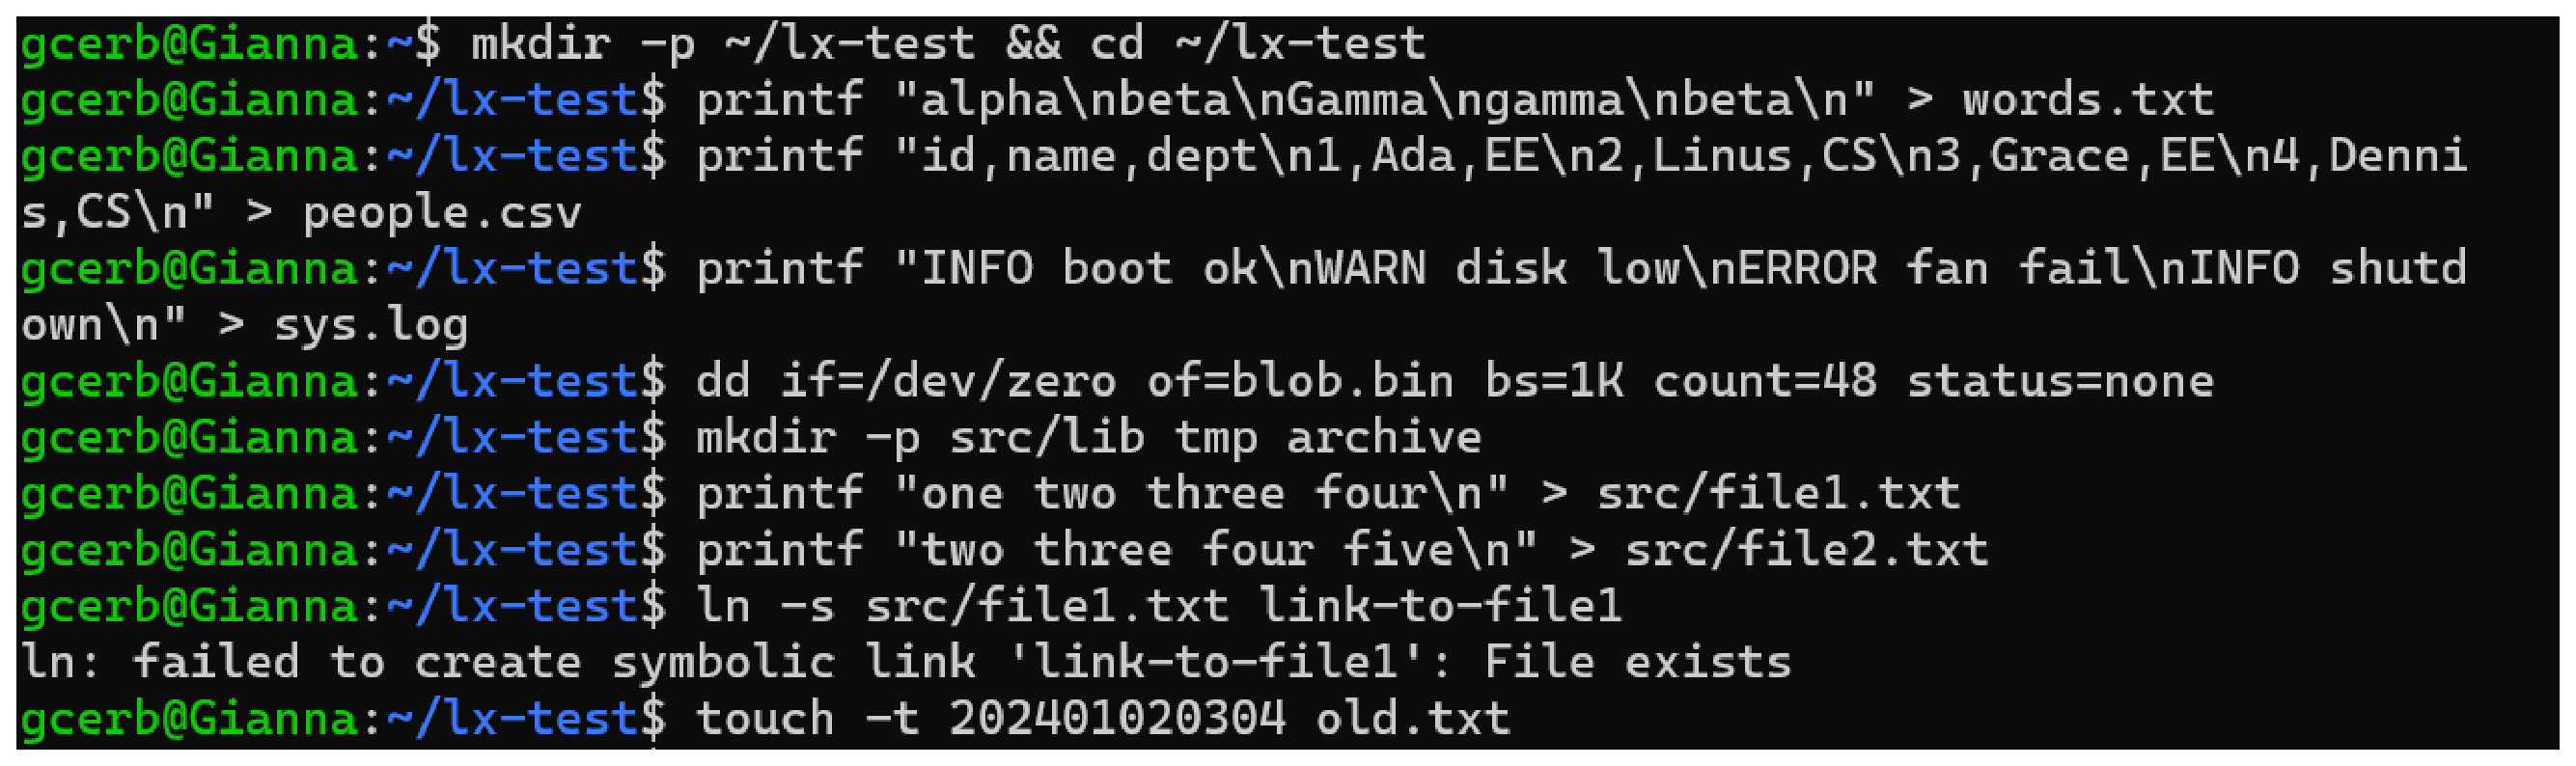
\includegraphics[width=1.0\textwidth]{eps/LinuxBash.eps}
    \caption{Screenshot of Linux Bash commands executed.}
    \label{fig:LinuxBash}
\end{figure}

\section{Linux Problem Set}

\subsection*{A) Navigation \& File Ops}
\begin{verbatim}
1.  pwd
2.  ls -A1
3.  [ -d tmp ] && cp -v src/file1.txt tmp/
4.  mv -v --preserve=timestamps old.txt archive/
5.  touch notes.md  (only if not exists: test -e notes.md || 
(continued) touch notes.md)
6.  du -sh src
\end{verbatim}

\subsection*{B) Viewing \& Searching}
\begin{verbatim}
7.  nl sys.log
8.  grep 'ERROR' sys.log
9.  tr '[:upper:]' '[:lower:]' < words.txt | tr -c '[:alnum:]' '[\n*]' | 
(continued) sort -u | wc -l
10. grep -i '^g' words.txt
11. head -n 2 people.csv
12. tail -n 3 -f sys.log
\end{verbatim}

\subsection*{C) Text Processing}
\begin{verbatim}
13. cut -d',' -f2 people.csv | tail -n +2
14. sort -f words.txt | uniq
15. sed -i.bak 's/three/3/g' src/*
16. wc src/*.txt
\end{verbatim}

\subsection*{D) Permissions \& Ownership}
\begin{verbatim}
17. chmod 700 tmp/
18. chmod -R g+x src/lib
19. stat -c "%a" src/file2.txt
20. chattr +a notes.md
\end{verbatim}

\subsection*{E) Links \& Find}
\begin{verbatim}
21. test -L link-to-file1 && readlink -f link-to-file1
22. find . -type f -size +40k
23. find tmp/ -type f -mmin -10 -exec ls -lh {} +
\end{verbatim}

\subsection*{F) Processes \& Job Control}
\begin{verbatim}
24. pstree -p
25. sleep 120 & echo $!
26. pkill -TERM -u "$USER" sleep
27. ps -eo pid,comm,%mem --sort=-%mem | head -n 6
\end{verbatim}

\subsection*{G) Archiving \& Compression}
\begin{verbatim}
28. tar -czf src.tgz src/
29. tar -tzf src.tgz
30. tar -xzf src.tgz -C tmp src/file2.txt
\end{verbatim}

\subsection*{H) Networking \& System Info}
\begin{verbatim}
31. ss -ltnp
32. ip route show default
33. uname -srm
34. last -n 5
\end{verbatim}

\subsection*{I) Package \& Services (Debian/Ubuntu)}
\begin{verbatim}
35. dpkg -s coreutils | grep Version
36. apt-cache search ripgrep
37. systemctl is-active cron
\end{verbatim}

\subsection*{J) Bash \& Scripting}
\begin{verbatim}
38. for f in src/*.txt; do echo "$f: $(cat "$f")"; done
39. awk -F',' '$3=="CS" && NR>1 {print > "cs.txt"}' people.csv
40. export X=42; echo $X; unset X
\end{verbatim}






